% Options for packages loaded elsewhere
\PassOptionsToPackage{unicode}{hyperref}
\PassOptionsToPackage{hyphens}{url}
%
\documentclass[
  12,
  a4paper,
]{report}
\usepackage{amsmath,amssymb}
\usepackage{iftex}
\ifPDFTeX
  \usepackage[T1]{fontenc}
  \usepackage[utf8]{inputenc}
  \usepackage{textcomp} % provide euro and other symbols
\else % if luatex or xetex
  \usepackage{unicode-math} % this also loads fontspec
  \defaultfontfeatures{Scale=MatchLowercase}
  \defaultfontfeatures[\rmfamily]{Ligatures=TeX,Scale=1}
\fi
\usepackage{lmodern}
\ifPDFTeX\else
  % xetex/luatex font selection
\fi
% Use upquote if available, for straight quotes in verbatim environments
\IfFileExists{upquote.sty}{\usepackage{upquote}}{}
\IfFileExists{microtype.sty}{% use microtype if available
  \usepackage[]{microtype}
  \UseMicrotypeSet[protrusion]{basicmath} % disable protrusion for tt fonts
}{}
\makeatletter
\@ifundefined{KOMAClassName}{% if non-KOMA class
  \IfFileExists{parskip.sty}{%
    \usepackage{parskip}
  }{% else
    \setlength{\parindent}{0pt}
    \setlength{\parskip}{6pt plus 2pt minus 1pt}}
}{% if KOMA class
  \KOMAoptions{parskip=half}}
\makeatother
\usepackage{xcolor}
\usepackage[margin=1in]{geometry}
\usepackage{color}
\usepackage{fancyvrb}
\newcommand{\VerbBar}{|}
\newcommand{\VERB}{\Verb[commandchars=\\\{\}]}
\DefineVerbatimEnvironment{Highlighting}{Verbatim}{commandchars=\\\{\}}
% Add ',fontsize=\small' for more characters per line
\usepackage{framed}
\definecolor{shadecolor}{RGB}{248,248,248}
\newenvironment{Shaded}{\begin{snugshade}}{\end{snugshade}}
\newcommand{\AlertTok}[1]{\textcolor[rgb]{0.94,0.16,0.16}{#1}}
\newcommand{\AnnotationTok}[1]{\textcolor[rgb]{0.56,0.35,0.01}{\textbf{\textit{#1}}}}
\newcommand{\AttributeTok}[1]{\textcolor[rgb]{0.13,0.29,0.53}{#1}}
\newcommand{\BaseNTok}[1]{\textcolor[rgb]{0.00,0.00,0.81}{#1}}
\newcommand{\BuiltInTok}[1]{#1}
\newcommand{\CharTok}[1]{\textcolor[rgb]{0.31,0.60,0.02}{#1}}
\newcommand{\CommentTok}[1]{\textcolor[rgb]{0.56,0.35,0.01}{\textit{#1}}}
\newcommand{\CommentVarTok}[1]{\textcolor[rgb]{0.56,0.35,0.01}{\textbf{\textit{#1}}}}
\newcommand{\ConstantTok}[1]{\textcolor[rgb]{0.56,0.35,0.01}{#1}}
\newcommand{\ControlFlowTok}[1]{\textcolor[rgb]{0.13,0.29,0.53}{\textbf{#1}}}
\newcommand{\DataTypeTok}[1]{\textcolor[rgb]{0.13,0.29,0.53}{#1}}
\newcommand{\DecValTok}[1]{\textcolor[rgb]{0.00,0.00,0.81}{#1}}
\newcommand{\DocumentationTok}[1]{\textcolor[rgb]{0.56,0.35,0.01}{\textbf{\textit{#1}}}}
\newcommand{\ErrorTok}[1]{\textcolor[rgb]{0.64,0.00,0.00}{\textbf{#1}}}
\newcommand{\ExtensionTok}[1]{#1}
\newcommand{\FloatTok}[1]{\textcolor[rgb]{0.00,0.00,0.81}{#1}}
\newcommand{\FunctionTok}[1]{\textcolor[rgb]{0.13,0.29,0.53}{\textbf{#1}}}
\newcommand{\ImportTok}[1]{#1}
\newcommand{\InformationTok}[1]{\textcolor[rgb]{0.56,0.35,0.01}{\textbf{\textit{#1}}}}
\newcommand{\KeywordTok}[1]{\textcolor[rgb]{0.13,0.29,0.53}{\textbf{#1}}}
\newcommand{\NormalTok}[1]{#1}
\newcommand{\OperatorTok}[1]{\textcolor[rgb]{0.81,0.36,0.00}{\textbf{#1}}}
\newcommand{\OtherTok}[1]{\textcolor[rgb]{0.56,0.35,0.01}{#1}}
\newcommand{\PreprocessorTok}[1]{\textcolor[rgb]{0.56,0.35,0.01}{\textit{#1}}}
\newcommand{\RegionMarkerTok}[1]{#1}
\newcommand{\SpecialCharTok}[1]{\textcolor[rgb]{0.81,0.36,0.00}{\textbf{#1}}}
\newcommand{\SpecialStringTok}[1]{\textcolor[rgb]{0.31,0.60,0.02}{#1}}
\newcommand{\StringTok}[1]{\textcolor[rgb]{0.31,0.60,0.02}{#1}}
\newcommand{\VariableTok}[1]{\textcolor[rgb]{0.00,0.00,0.00}{#1}}
\newcommand{\VerbatimStringTok}[1]{\textcolor[rgb]{0.31,0.60,0.02}{#1}}
\newcommand{\WarningTok}[1]{\textcolor[rgb]{0.56,0.35,0.01}{\textbf{\textit{#1}}}}
\usepackage{graphicx}
\makeatletter
\def\maxwidth{\ifdim\Gin@nat@width>\linewidth\linewidth\else\Gin@nat@width\fi}
\def\maxheight{\ifdim\Gin@nat@height>\textheight\textheight\else\Gin@nat@height\fi}
\makeatother
% Scale images if necessary, so that they will not overflow the page
% margins by default, and it is still possible to overwrite the defaults
% using explicit options in \includegraphics[width, height, ...]{}
\setkeys{Gin}{width=\maxwidth,height=\maxheight,keepaspectratio}
% Set default figure placement to htbp
\makeatletter
\def\fps@figure{htbp}
\makeatother
\setlength{\emergencystretch}{3em} % prevent overfull lines
\providecommand{\tightlist}{%
  \setlength{\itemsep}{0pt}\setlength{\parskip}{0pt}}
\setcounter{secnumdepth}{-\maxdimen} % remove section numbering
\ifLuaTeX
  \usepackage{selnolig}  % disable illegal ligatures
\fi
\IfFileExists{bookmark.sty}{\usepackage{bookmark}}{\usepackage{hyperref}}
\IfFileExists{xurl.sty}{\usepackage{xurl}}{} % add URL line breaks if available
\urlstyle{same}
\hypersetup{
  pdftitle={Cyber Crimes Trend in India, Fraud: The Major Motive.},
  pdfauthor={Jaswinderpal Singh Narinder Kumar},
  hidelinks,
  pdfcreator={LaTeX via pandoc}}

\title{\textbf{Cyber Crimes Trend in India, Fraud: The Major Motive.}}
\usepackage{etoolbox}
\makeatletter
\providecommand{\subtitle}[1]{% add subtitle to \maketitle
  \apptocmd{\@title}{\par {\large #1 \par}}{}{}
}
\makeatother
\subtitle{\textbf{Project Report }}
\author{\textbf{Jaswinderpal Singh \n   Narinder Kumar}}
\date{23 March 2023}

\begin{document}
\maketitle

\hypertarget{abstract}{%
\chapter{Abstract}\label{abstract}}

Cyber Crime is any kind of criminal activity that involves the use of
computers, networks, or the internet for the exploitation of data and
resources. Examples include hacking, identity theft, phishing scams, and
distributing malware etc. With the advancements in technology, increased
accessibility of the internet to rural areas, the criminal activities
are also getting digital and more advanced.\\
Situation is getting worse with every passing year and at the same time
lack of awareness in terms of digital literacy is still there.
Currently, the active internet users in India are more than 50\% of the
country's population. The Cyber Crimes started increasing rapidly by the
years 2015-2016. Lack of Digital Literacy and Cyber Safety are some of
the reasons. Phishing, Identity Theft, Computer Related Offenses,
Frauds, Cyber-Bullying, Spamming, data leaks etc. are major Cyber Crimes
on the increase in India.\\
Here, the objective is to analyze the year-wise trend and future
prediction of the number of cyber crimes registered in India using the
data from 2002 - 2021. Some state wise comparisons are done, keeping the
population variation of the states under consideration. Major Cyber
Crime Motive is identified and States with similar crime incidence rates
are divided into clusters using Statistical Cluster Analysis Techniques.

\textbf{Keywords}: Cyber Crimes, Phishing, Malware, Fraud, Statistics,
Cluster Analysis

\hypertarget{introduction}{%
\chapter{Introduction}\label{introduction}}

\hypertarget{cyber-crimes}{%
\section{Cyber Crimes}\label{cyber-crimes}}

Cybercrime refers to any criminal activity that involves the use of
computers, networks, or the internet. Examples include hacking, identity
theft, phishing scams, and distributing malware etc.

Cyber crimes are a new class of crimes rapidly increasing due to
extensive use of Internet and I.T. enabled services.

\hypertarget{major-cyber-crimes-in-india}{%
\subsection{Major Cyber Crimes in
India}\label{major-cyber-crimes-in-india}}

Some major cyber crimes in India include:\\
1. \emph{Hacking:} Unauthorized access to computer systems, networks, or
websites to steal sensitive information or disrupt operations.\\
2. \emph{Phishing:} Attempts to trick individuals into providing
personal or financial information through fake emails or websites.\\
3. \emph{Identity Theft:} Using someone else's personal information to
commit fraud or other crimes.\\
4. \emph{Fraud:} Using the internet to scam people out of their money or
personal information.\\
5. \emph{Cyberstalking:} Harassment or bullying through electronic
means.\\
6. \emph{Child pornography:} Using the internet to distribute or view
child pornography.\\
7. \emph{Ransomware:} A type of malware that encrypts a victim's files
and demands payment to restore access.\\
8. \emph{Crypto jacking:} Unauthorized use of someone's computer or
device to mine cryptocurrency.\\
9. \emph{Distributed Denial of Service (DDoS) attacks:} Overwhelming a
website or network with traffic to make it unavailable. 10.
\emph{Spamming:} Sending unsolicited messages through email or other
means.

These are some major cyber crimes reported in India, but there can be
various other types of cyber-attacks that are emerging with technology
advancements.

\hypertarget{cyber-crimes-in-india-statistics-and-data-visualization}{%
\chapter{Cyber Crimes in India: Statistics and Data
Visualization}\label{cyber-crimes-in-india-statistics-and-data-visualization}}

\hypertarget{cyber-crimes-state-wise}{%
\section{Cyber Crimes State-Wise:}\label{cyber-crimes-state-wise}}

\hypertarget{year-2020}{%
\subsection{Year 2020}\label{year-2020}}

\begin{Shaded}
\begin{Highlighting}[]
\FunctionTok{rm}\NormalTok{(}\AttributeTok{list =} \FunctionTok{ls}\NormalTok{())}
\FunctionTok{source}\NormalTok{(}\StringTok{"viz2021.R"}\NormalTok{)}

\NormalTok{barst2020}
\end{Highlighting}
\end{Shaded}

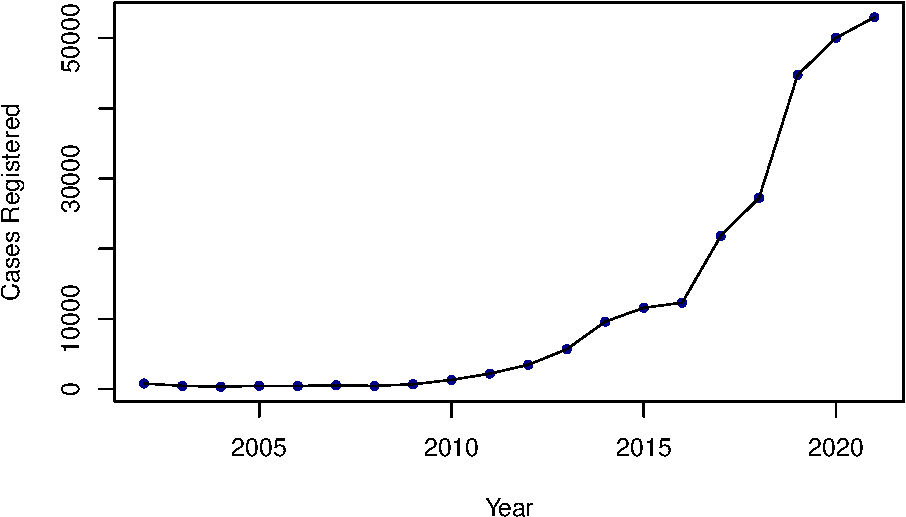
\includegraphics{ncrb_report_files/figure-latex/unnamed-chunk-1-1.pdf}

The above figure shows the highest number of cases being registered in
Uttar Pradesh, followed by Karnataka, Maharashtra and Telangana. But one
must note that the population in these states may vary. So to get a
better comparison, rates can be calculated, which gives the cyber crime
cases registered in the state per 1 lakh population. Mid year projected
population for each state for the year 2021 is available. Hence the
Cyber Crime Rate can be calculated as:\\
\[Rate = \frac{No. \ of \ cases \ registered }{Mid \ year \ projected \ population \ (in \ lakhs)}\]

\begin{Shaded}
\begin{Highlighting}[]
\NormalTok{barst2020r}
\end{Highlighting}
\end{Shaded}

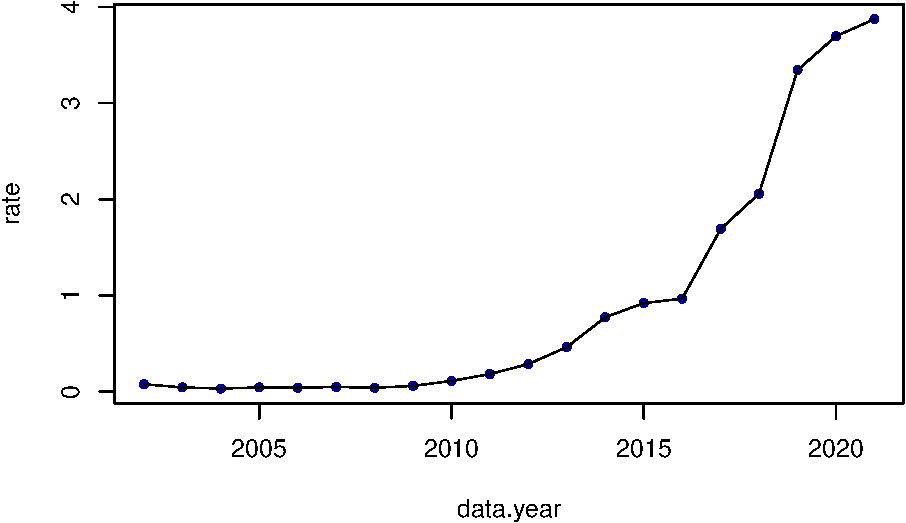
\includegraphics{ncrb_report_files/figure-latex/unnamed-chunk-2-1.pdf}
As far as the rates are concerned, Karnataka and Telangana emerged as
the states with highest cyber crime rates followed by Assam, Uttar
Pradesh and Maharashtra.

\begin{Shaded}
\begin{Highlighting}[]
\NormalTok{major\_states20 }\OtherTok{=}\NormalTok{ df}\SpecialCharTok{$}\NormalTok{cases\_reg2020[ }\FunctionTok{which}\NormalTok{(df}\SpecialCharTok{$}\NormalTok{state }\SpecialCharTok{\%in\%} \FunctionTok{c}\NormalTok{(}\StringTok{"Telangana"}\NormalTok{, }\StringTok{"Assam"}\NormalTok{, }
                            \StringTok{"Uttar Pradesh"}\NormalTok{, }\StringTok{"Karnataka"}\NormalTok{, }\StringTok{"Maharashtra"}\NormalTok{) ) ]}
\FunctionTok{sum}\NormalTok{(major\_states20)}\SpecialCharTok{/}\NormalTok{df[}\DecValTok{40}\NormalTok{,}\DecValTok{4}\NormalTok{]}
\end{Highlighting}
\end{Shaded}

\begin{verbatim}
## [1] 0.7172579
\end{verbatim}

\textbf{The above value indicates that almost 71.72579 \% of the total
cyber crimes reported in the country India in 2021 came only from the
five states: Telangana, Uttar Pradesh, Karnataka, Maharashtra and
Assam.}

\hypertarget{year-2021}{%
\subsection{Year 2021}\label{year-2021}}

\begin{Shaded}
\begin{Highlighting}[]
\NormalTok{barst2021}
\end{Highlighting}
\end{Shaded}

\includegraphics{ncrb_report_files/figure-latex/unnamed-chunk-4-1.pdf}

From the above figure it looks like Telangana tops the Cyber Crimes
tally followed by Uttar Pradesh and Karnataka in 2021. But for better
comparison, let us see the Cyber Crime Rates, i.e.~Cyber Crimes in a
State per 1 lakh population.

\begin{Shaded}
\begin{Highlighting}[]
\NormalTok{barst2021r}
\end{Highlighting}
\end{Shaded}

\includegraphics{ncrb_report_files/figure-latex/unnamed-chunk-5-1.pdf}

Now, from here it is evident that infact Telangana is the state with
highest cyber crime rate of 27.28 cases per 1 lakh population, followed
by Assam and Karnataka with rates 13.78 and 12.15 respectively.

\begin{Shaded}
\begin{Highlighting}[]
\NormalTok{major\_states21 }\OtherTok{=}\NormalTok{ df}\SpecialCharTok{$}\NormalTok{cases\_reg2021[ }\FunctionTok{which}\NormalTok{(df}\SpecialCharTok{$}\NormalTok{state }\SpecialCharTok{\%in\%} \FunctionTok{c}\NormalTok{(}\StringTok{"Telangana"}\NormalTok{, }\StringTok{"Assam"}\NormalTok{, }
                            \StringTok{"Uttar Pradesh"}\NormalTok{, }\StringTok{"Karnataka"}\NormalTok{, }\StringTok{"Maharashtra"}\NormalTok{) ) ]}
\FunctionTok{sum}\NormalTok{(major\_states21)}\SpecialCharTok{/}\NormalTok{df[}\DecValTok{40}\NormalTok{,}\DecValTok{5}\NormalTok{]}
\end{Highlighting}
\end{Shaded}

\begin{verbatim}
## [1] 0.7112168
\end{verbatim}

\textbf{The above value indicates that almost 71.12168 \% of the total
cyber crimes reported in the country India in 2021 came only from the
five states: Telangana, Uttar Pradesh, Karnataka, Maharashtra and Assam.
However, they together contributed almost 36\% of the Indian Population}

\hypertarget{cyber-crimes-trend-major-states}{%
\subsection{Cyber Crimes Trend: Major
States}\label{cyber-crimes-trend-major-states}}

These States can be analyzed further based on last 5 years as follows:

\begin{Shaded}
\begin{Highlighting}[]
\NormalTok{j }\OtherTok{=} \DecValTok{1}
\ControlFlowTok{for}\NormalTok{ (i }\ControlFlowTok{in}\NormalTok{ statelist) \{}
  \FunctionTok{cat}\NormalTok{(}\StringTok{"}\SpecialCharTok{\textbackslash{}n}\StringTok{"}\NormalTok{,nam[j],}\StringTok{"}\SpecialCharTok{\textbackslash{}n}\StringTok{"}\NormalTok{)}
  \FunctionTok{show}\NormalTok{(}\FunctionTok{trend\_plot}\NormalTok{(i,  }\FunctionTok{paste}\NormalTok{(}\StringTok{"Cyber Crime Trend"}\NormalTok{,nam[j],}\StringTok{"2017 {-} 2021"}\NormalTok{), i}\SpecialCharTok{$}\NormalTok{cases) )}
  \FunctionTok{cat}\NormalTok{(}\StringTok{"}\SpecialCharTok{\textbackslash{}n}\StringTok{"}\NormalTok{)}
  \FunctionTok{show}\NormalTok{(}\FunctionTok{trend\_plot}\NormalTok{(i,  }\FunctionTok{paste}\NormalTok{(}\StringTok{"Cyber Crime Rates Trend"}\NormalTok{,nam[j],}\StringTok{"2017 {-} 2021"}\NormalTok{), i}\SpecialCharTok{$}\NormalTok{rates) )}
  \FunctionTok{cat}\NormalTok{(}\StringTok{"}\SpecialCharTok{\textbackslash{}n}\StringTok{"}\NormalTok{)}
\NormalTok{  j }\OtherTok{=}\NormalTok{ j}\SpecialCharTok{+}\DecValTok{1}
\NormalTok{\}}
\end{Highlighting}
\end{Shaded}

\begin{verbatim}
## 
##  Telangana
\end{verbatim}

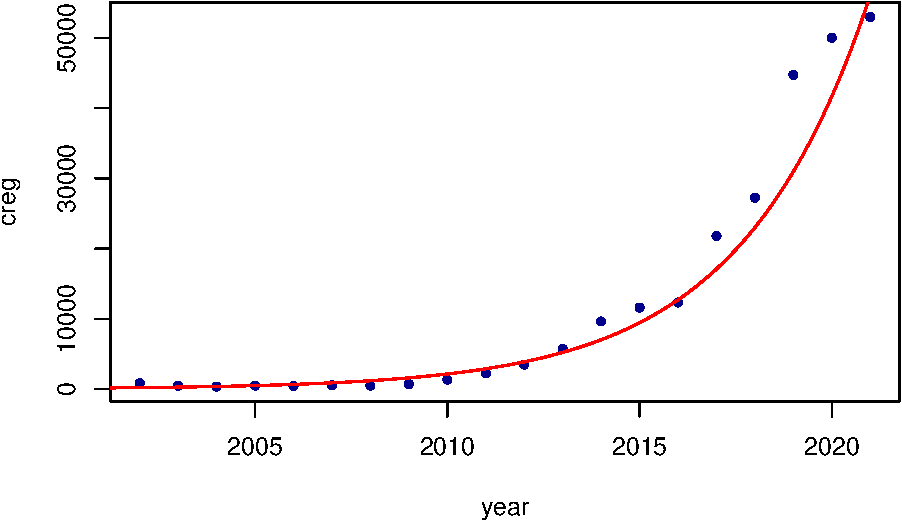
\includegraphics{ncrb_report_files/figure-latex/unnamed-chunk-7-1.pdf}
\includegraphics{ncrb_report_files/figure-latex/unnamed-chunk-7-2.pdf}

\begin{verbatim}
## 
## 
##  Karnataka
\end{verbatim}

\includegraphics{ncrb_report_files/figure-latex/unnamed-chunk-7-3.pdf}
\includegraphics{ncrb_report_files/figure-latex/unnamed-chunk-7-4.pdf}

\begin{verbatim}
## 
## 
##  Maharashtra
\end{verbatim}

\includegraphics{ncrb_report_files/figure-latex/unnamed-chunk-7-5.pdf}
\includegraphics{ncrb_report_files/figure-latex/unnamed-chunk-7-6.pdf}

\begin{verbatim}
## 
## 
##  Assam
\end{verbatim}

\includegraphics{ncrb_report_files/figure-latex/unnamed-chunk-7-7.pdf}
\includegraphics{ncrb_report_files/figure-latex/unnamed-chunk-7-8.pdf}

\begin{verbatim}
## 
## 
##  Uttar Pradesh
\end{verbatim}

\includegraphics{ncrb_report_files/figure-latex/unnamed-chunk-7-9.pdf}
\includegraphics{ncrb_report_files/figure-latex/unnamed-chunk-7-10.pdf}

Now, it is evident from that the states of Assam and Telangana are
showing rapid increasing trend in Cyber Crimes over the last 5 years.
However, Uttar Pradesh and Karnataka are registering some lesser number
of cases as compared to previous years. The state of Maharashtra is
slowly registering more number of cases as compared to previous years.

\hypertarget{cyber-crimes-u.t.---wise}{%
\section{Cyber Crimes U.T. - wise}\label{cyber-crimes-u.t.---wise}}

Further, Similar things can be analyzed for the Union Territories also.

\begin{Shaded}
\begin{Highlighting}[]
\NormalTok{barut2020\_21}
\end{Highlighting}
\end{Shaded}

\includegraphics{ncrb_report_files/figure-latex/unnamed-chunk-8-1.pdf}

In terms of numbers, the Union Territory of Delhi registered the most
356 cyber crime cases in 2021, followed by Jammu\&Kashmir and Chandigarh
with 154 ans 15 cases respectively. Also, \textbf{the cases in Delhi are
more than double in 2021 from 2020.} However, in terms of rates, the
picture is somewhat like this in all the Union Territories:

\begin{Shaded}
\begin{Highlighting}[]
\NormalTok{barut2020\_21r}
\end{Highlighting}
\end{Shaded}

\includegraphics{ncrb_report_files/figure-latex/unnamed-chunk-9-1.pdf}

\hypertarget{cyber-crime-trend-india}{%
\section{Cyber Crime Trend India}\label{cyber-crime-trend-india}}

\begin{Shaded}
\begin{Highlighting}[]
\FunctionTok{source}\NormalTok{(}\StringTok{"cybertrend.R"}\NormalTok{)}
\NormalTok{cyber\_trend}
\end{Highlighting}
\end{Shaded}

\includegraphics{ncrb_report_files/figure-latex/unnamed-chunk-10-1.pdf}

Now, the above plot shows the Trend for the number of Total Cyber Crimes
registered in overall India from the year 2002 - 2021.

Now, it is evident from the plot, that India registered more than
\textbf{4 times} cyber crimes in 2021 as compared to 2016.

Also, in a span of an year, India registered \textbf{1.5 times} more
Cyber Crime cases in 2018 from 2017. And if we see 2018 from 2016, then
the registration of the cases is \textbf{just above double}.

Also, one may note that initially, from the years 2002 - 2009, the cases
registered were much much lower due to the fact that the internet was
not that cheaply and easily accessible for the. people of India.\\
But from the year 2016 to 2017, the cyber crimes were \textbf{almost
doubled} due to the fact that in this year the telecom sector in India
experienced drastic changes with the entry of Jio in the Telecom Market.
To tackle with their bussiness strategies, other telecom networks
reduced the data charges to a huge extent, leading to a very large
increase in the Internet accessibility among the Indian Population.

Also, it is a fact that the population of India also varied in these
years. For that matter, we can observe the Cyber Crime Rgistration Rate
of India from 2002 - 2021 as follows:

\begin{Shaded}
\begin{Highlighting}[]
\NormalTok{cyber\_trendr}
\end{Highlighting}
\end{Shaded}

\includegraphics{ncrb_report_files/figure-latex/unnamed-chunk-11-1.pdf}

The cyber crime rate prediction for the coming years can be done using
the following fitted model:

\[\log(Y_t) = -4.26073 + 0.28345 \ t\] or
\[Y_t = \exp(-4.26073 + 0.28345 \ t)\] where:\\
t \(\geq\) 1\\
\(Y_t\) : Predicted Cyber Crime Rate in India for the year
\((2001 + t)\)

\begin{Shaded}
\begin{Highlighting}[]
\FunctionTok{summary}\NormalTok{(model4)}
\end{Highlighting}
\end{Shaded}

\begin{verbatim}
## 
## Call:
## lm(formula = log(rate) ~ t)
## 
## Residuals:
##      Min       1Q   Median       3Q      Max 
## -0.93734 -0.29522 -0.01532  0.22008  1.41202 
## 
## Coefficients:
##             Estimate Std. Error t value Pr(>|t|)    
## (Intercept) -4.26073    0.24395  -17.47 9.85e-13 ***
## t            0.28345    0.02036   13.92 4.47e-11 ***
## ---
## Signif. codes:  0 '***' 0.001 '**' 0.01 '*' 0.05 '.' 0.1 ' ' 1
## 
## Residual standard error: 0.5251 on 18 degrees of freedom
## Multiple R-squared:  0.915,  Adjusted R-squared:  0.9103 
## F-statistic: 193.7 on 1 and 18 DF,  p-value: 4.475e-11
\end{verbatim}

Clearly, from the summary of the model, it is evident that the values of
\(R^2\) and Adjusted \(R^2\) do not differ much. Here t denotes the time
index. t = 2 corresponds to the year 2002, upto so on t = 20 for the
year 2021. The parameter estimates are coming out to be highly
significant.

\begin{Shaded}
\begin{Highlighting}[]
\NormalTok{fitplot}
\end{Highlighting}
\end{Shaded}

\includegraphics{ncrb_report_files/figure-latex/unnamed-chunk-13-1.pdf}

The Cyber Crime Rates predicted for the coming years using the above
model are:

\begin{Shaded}
\begin{Highlighting}[]
\NormalTok{rate.prediction}
\end{Highlighting}
\end{Shaded}

\begin{verbatim}
##    year predicted_rate
## 1  2022          5.429
## 2  2023          7.209
## 3  2024          9.571
## 4  2025         12.707
## 5  2026         16.871
## 6  2027         22.400
## 7  2028         29.741
## 8  2029         39.488
## 9  2030         52.428
## 10 2031         69.609
\end{verbatim}

To get a more clear idea about the previous year comparison, percentage
increase in the cases can be calculated using the formula:

\[ Percentage \ Increase =  \frac{Current \ Value - Previous \ Value}{Previous \ value} *100\]
From the Percentage Increase plot, following facts can be noted:

\begin{itemize}
\tightlist
\item
  India registered 5.87\% more cyber crimes in 2020 as compared to
  2021.\\
\item
  It must be noted that the any dip in the graph does not mean decrease
  in the crimes, rather it means that there is less percentage increase
  in the cases as compared to previous year. However any point below
  zero, i.e.~negative percentage increase indicates that there are
  lesser number of cases from the previous year.
\end{itemize}

\begin{Shaded}
\begin{Highlighting}[]
\NormalTok{cyber\_trendp}
\end{Highlighting}
\end{Shaded}

\includegraphics{ncrb_report_files/figure-latex/unnamed-chunk-15-1.pdf}

\textbf{Internet user-base of India}

\begin{Shaded}
\begin{Highlighting}[]
\NormalTok{net\_usep}
\end{Highlighting}
\end{Shaded}

\includegraphics{ncrb_report_files/figure-latex/unnamed-chunk-16-1.pdf}

\hypertarget{references}{%
\section{References:}\label{references}}

\begin{itemize}
\tightlist
\item
  Cyber Crimes data: National Crime Records Bureau (NCRB), Ministry of
  Home Affairs, Govt. of India.\\
\item
  Individuals using the Internet (\% of population) - India:
  International Telecommunication Union ( ITU ) World
  Telecommunication/ICT Indicators Database
\end{itemize}

\hypertarget{cyber-crime-motives}{%
\chapter{Cyber Crime Motives}\label{cyber-crime-motives}}

For the various cyber crimes happening in India, the data for the
motives behind them is available, which can be observed as follows:

\hypertarget{cyber-crime-motives-year-wise}{%
\section{Cyber Crime Motives Year
Wise}\label{cyber-crime-motives-year-wise}}

\hypertarget{year-2020-1}{%
\subsection{Year 2020}\label{year-2020-1}}

From the following diagram, it is evident that, in 2020, the major
motive behind the cyber crimes in India was Fraud, contributing to 60\%
of the total cyber crimes in India.

\begin{Shaded}
\begin{Highlighting}[]
\FunctionTok{source}\NormalTok{(}\StringTok{"cybermotives.R"}\NormalTok{)}
\NormalTok{motives2020}
\end{Highlighting}
\end{Shaded}

\includegraphics{ncrb_report_files/figure-latex/unnamed-chunk-17-1.pdf}

\hypertarget{year-2021-1}{%
\subsection{Year 2021}\label{year-2021-1}}

Again in the next consecutive year 2021, it can be seen that Fraud
emerges as the major cyber crime motive in India, contributing to
60.24\% of the total cyber crimes in the country.

\begin{Shaded}
\begin{Highlighting}[]
\NormalTok{motives2021}
\end{Highlighting}
\end{Shaded}

\includegraphics{ncrb_report_files/figure-latex/unnamed-chunk-18-1.pdf}

\hypertarget{cluster-analysis}{%
\section{Cluster Analysis}\label{cluster-analysis}}

For the fraud cases, different states of India are divided into
different clusters based on the fraction of fraud in the total cyber
crimes in that states for the years 2017 to 2021.

States are divided into 4 clusters, K-Means Clustering is implemented as
Non-Hierarchical cluster analysis and Agglomerative \& Divisive
Techniques are also implemented under Hierarchical cluster anlaysis.

\hypertarget{distance-matrix-calculations}{%
\subsection{Distance Matrix
Calculations}\label{distance-matrix-calculations}}

Data has been scaled to centre 0, and unit variability of each year rate
(Variables).

\begin{Shaded}
\begin{Highlighting}[]
\FunctionTok{source}\NormalTok{(}\StringTok{"clusterana.R"}\NormalTok{)}
\end{Highlighting}
\end{Shaded}

\begin{verbatim}
## Welcome! Want to learn more? See two factoextra-related books at https://goo.gl/ve3WBa
\end{verbatim}

\begin{Shaded}
\begin{Highlighting}[]
\NormalTok{dist[}\DecValTok{1}\SpecialCharTok{:}\DecValTok{3}\NormalTok{, }\DecValTok{1}\SpecialCharTok{:}\DecValTok{3}\NormalTok{]}
\end{Highlighting}
\end{Shaded}

\begin{verbatim}
##                   Andhra Pradesh Arunachal Pradesh    Assam
## Andhra Pradesh          0.000000          3.937371 4.223798
## Arunachal Pradesh       3.937371          0.000000 3.029010
## Assam                   4.223798          3.029010 0.000000
\end{verbatim}

These are some part of the 28x28 distance matrix of states. This
distance matrix can be easily visualized in the following manner:

\begin{Shaded}
\begin{Highlighting}[]
\NormalTok{displot}
\end{Highlighting}
\end{Shaded}

\includegraphics{ncrb_report_files/figure-latex/unnamed-chunk-20-1.pdf}

The above plot shows the states with most similarity with dark reddish
shade to less similarity with light red shades upto dark blue shades
with least similar.

\hypertarget{k-means-clustering-non-hierarchical}{%
\subsection{K-Means Clustering
(Non-Hierarchical)}\label{k-means-clustering-non-hierarchical}}

To determine the optimum number of clusters, consider the following plot
of number of clusters v/s Total within sum of squares.

\begin{Shaded}
\begin{Highlighting}[]
\NormalTok{wssplot}
\end{Highlighting}
\end{Shaded}

\includegraphics{ncrb_report_files/figure-latex/unnamed-chunk-21-1.pdf}

According to the above plot, the Total within sum of squares starts
flattening after k = 2.

We now proceed with \textbf{K-Means clustering} with 2 clusters.

\begin{Shaded}
\begin{Highlighting}[]
\NormalTok{km.res}\SpecialCharTok{$}\NormalTok{cluster}
\end{Highlighting}
\end{Shaded}

\begin{verbatim}
##    Andhra Pradesh Arunachal Pradesh             Assam             Bihar 
##                 2                 1                 1                 2 
##      Chhattisgarh               Goa           Gujarat           Haryana 
##                 1                 2                 2                 1 
##  Himachal Pradesh         Jharkhand         Karnataka            Kerala 
##                 1                 2                 2                 1 
##    Madhya Pradesh       Maharashtra           Manipur         Meghalaya 
##                 1                 2                 1                 2 
##           Mizoram          Nagaland            Odisha            Punjab 
##                 1                 1                 2                 1 
##         Rajasthan            Sikkim        Tamil Nadu         Telangana 
##                 1                 1                 1                 2 
##           Tripura     Uttar Pradesh       Uttarakhand       West Bengal 
##                 1                 1                 1                 1
\end{verbatim}

This is the required clustering of 28 states into 2 clusters.

To have a better picture of the clusters, a look on the cluster plot
will be helpful:

\hypertarget{cluster-plot}{%
\subsubsection{Cluster Plot}\label{cluster-plot}}

\begin{Shaded}
\begin{Highlighting}[]
\NormalTok{clusplot}
\end{Highlighting}
\end{Shaded}

\includegraphics{ncrb_report_files/figure-latex/unnamed-chunk-23-1.pdf}

\begin{enumerate}
\def\labelenumi{\arabic{enumi}.}
\item
  As it is evident from the above cluster plot that the states with
  fewer fraud Cyber Crimes : Arunachal Pradesh and Nagaland are in one
  cluster.
\item
  However the states with extensive fraud rates: Karnataka,
  Bihar,Telangana, Jharkhand,Uttar Pradesh, Maharashtra etc. are in
  other cluster.
\end{enumerate}

\hypertarget{hierarchical-clustering}{%
\subsection{Hierarchical Clustering}\label{hierarchical-clustering}}

\hypertarget{agglomerative-clustering}{%
\subsubsection{Agglomerative
Clustering}\label{agglomerative-clustering}}

Also, Under the Hierarchical Clustering, using \textbf{Agglomerative
Custering} with \emph{Ward D2 Linkage}, the states are more likely to be
divided into 2 clusters.

The states with major fraction of the Fraud cases are in one Cluster:
Telangana, Jharkhand, Bihar etc.

However, the states with comparatively lesser number of frauds are in
the other cluster.

The cluster means are given by

\begin{Shaded}
\begin{Highlighting}[]
\NormalTok{cameans1 }\CommentTok{\# 1st cluster mean}
\end{Highlighting}
\end{Shaded}

\begin{verbatim}
##  rate2021  rate2020  rate2019  rate2018  rate2017 
## 0.5713483 0.6334256 0.5143662 0.4825693 0.4667825
\end{verbatim}

\begin{Shaded}
\begin{Highlighting}[]
\NormalTok{cameans2 }\CommentTok{\# 2nd Cluster mean}
\end{Highlighting}
\end{Shaded}

\begin{verbatim}
##  rate2021  rate2020  rate2019  rate2018  rate2017 
## 0.2367204 0.2255833 0.1450668 0.2455529 0.2827396
\end{verbatim}

\begin{Shaded}
\begin{Highlighting}[]
\NormalTok{aglodend}
\end{Highlighting}
\end{Shaded}

\includegraphics{ncrb_report_files/figure-latex/unnamed-chunk-25-1.pdf}

\begin{Shaded}
\begin{Highlighting}[]
\NormalTok{aglocp}
\end{Highlighting}
\end{Shaded}

\includegraphics{ncrb_report_files/figure-latex/unnamed-chunk-25-2.pdf}
Previously, for better demarkation, we applied K-Means clusteing for 4
clusters. However, under the Hierarchical Clustering, using
\textbf{Agglomerative Custering} with \emph{Ward D2 Linkage}, the states
are more likely to be divided into 2 clusters.

\hypertarget{divisive-clustering}{%
\subsubsection{Divisive Clustering}\label{divisive-clustering}}

On the other hand, if \textbf{Divisive Clustering} is applied, the two
main clusters so formed are given as follows:

\begin{Shaded}
\begin{Highlighting}[]
\NormalTok{dianadend}
\end{Highlighting}
\end{Shaded}

\includegraphics{ncrb_report_files/figure-latex/unnamed-chunk-26-1.pdf}

\end{document}
